\section{Computational infrastructure}

\begin{frame}{}
  \begin{center}
    \Large{\textbf{Behind the scenes}: software/data structures and
      open research practice.}
  \end{center}
\end{frame}


\begin{frame}{}

  Beyond the figures\footnote{... which are all reproducible, by the way.}

  \begin{itemize}
  \item<+-> Software: \textbf{infrastructure}
    (\href{http://bioconductor.org/packages/MSnbase}{\texttt{MSnbase}},
    \cite{Gatto:2012}), \textbf{dedicated machine learning}
    (\href{http://bioconductor.org/packages/pRoloc}{\texttt{pRoloc}},
    \cite{Gatto:2014a}), \textbf{interactive
      visualisation}\footnote{\url{https://lgatto.shinyapps.io/christoforou2015/}}
    (\href{http://bioconductor.org/packages/pRolocGUI}{\texttt{pRolocGUI}},
    \cite{pRolocGUI}) and \textbf{data}
    (\href{http://bioconductor.org/packages/pRolocdata}{\texttt{pRolocdata}},
    \cite{Gatto:2014a}) for spatial proteomics.
  \item<+-> The \href{http://bioconductor.org/}{\textbf{Bioconductor}}
    \citep{Huber:2015} ecosystem for high throughput biology data
    analysis and comprehension: \textbf{open source}, and
    \textbf{coordinated and collaborative\footnote{between and within
        domains/software} open development}, enabling
    \textbf{reproducible research}, enables understanding of the data
    (not a black box) and \textbf{drive scientific innovation}.
  \end{itemize}
\end{frame}


\begin{frame}
  \begin{figure}[h]
    \centering
    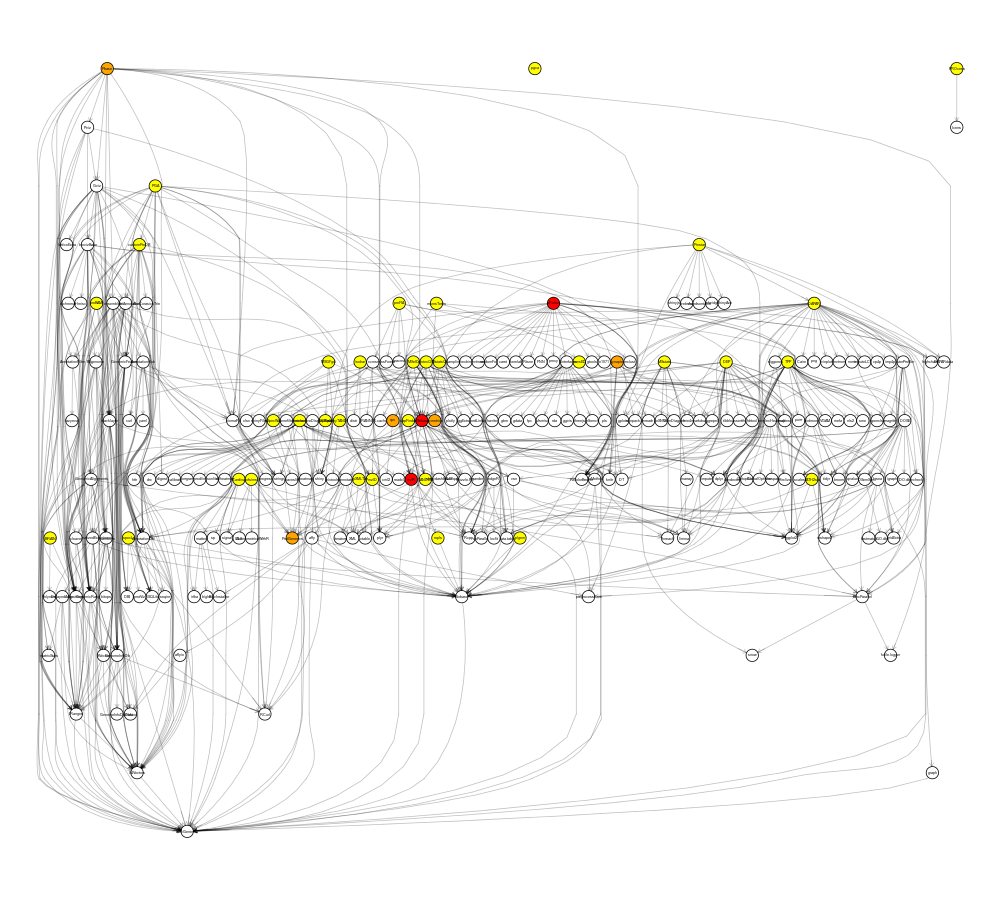
\includegraphics[width=.8\linewidth]{./figs_local/g.png}
    \caption{\textbf{Collaboration between packages}: Dependency graph
      containing 41 MS and proteomics-tagged packages (out of 100+)
      and their dependencies. }
  \end{figure}
\end{frame}

\begin{frame}{\textbf{MSnbase} example}

  \begin{figure}[h]
    \centering
    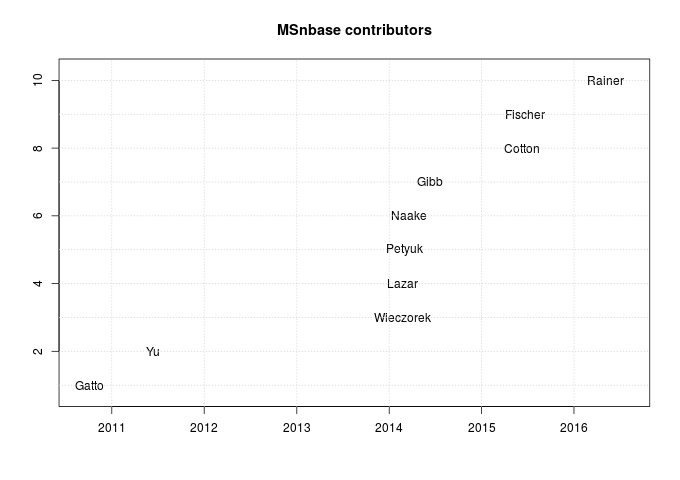
\includegraphics[width=.8\linewidth]{./Figures/msnbase-contributors-2.png}
    \caption{\textbf{Collaboration within packages}: Contributions to the
      \texttt{MSnbase} package (1220 downloads from unique IP
      addresses in January 2018) since its creation, the last one
      leading to \textbf{common proteomics/metabolomics
        infrastructure}. More details:
      \url{https://lgatto.github.io/msnbase-contribs/}}
    \label{fig:msnbase}
  \end{figure}

\end{frame}

\begin{frame}{Open research: open source software}
  \centering
  \begin{figure}
  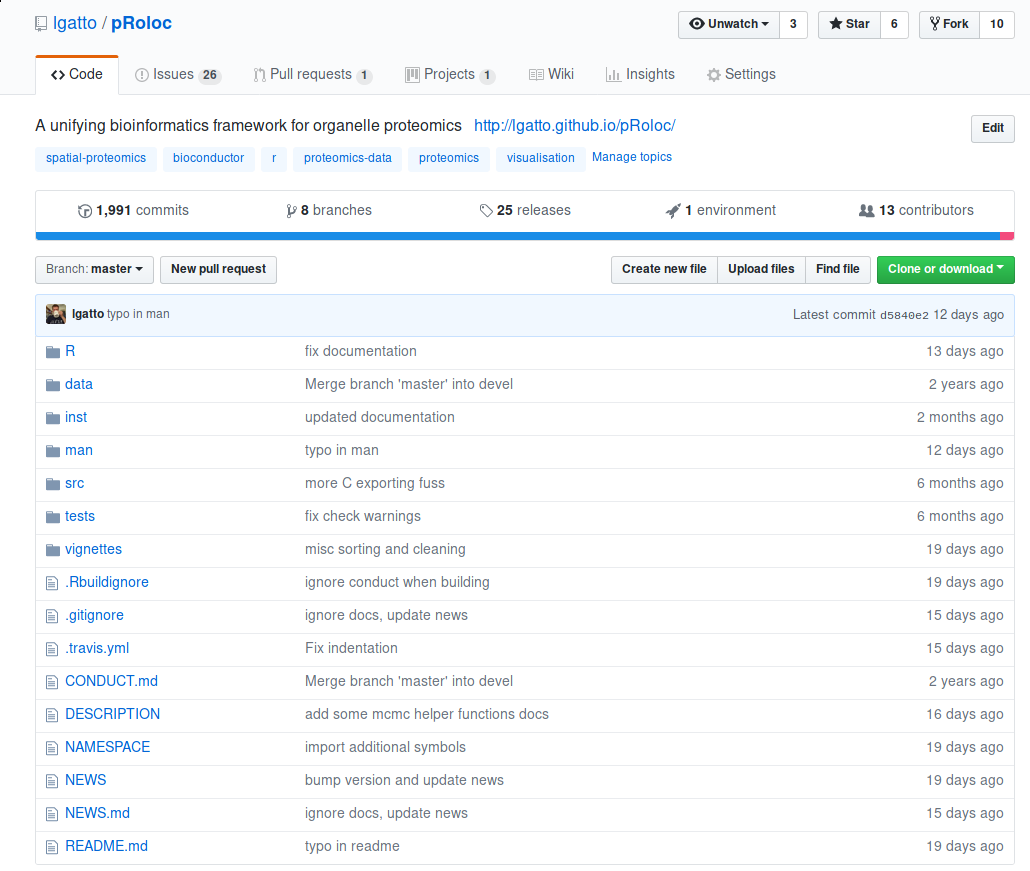
\includegraphics[width=.8\linewidth]{./figs_local/pRoloc_screen.png}
    \caption{Public repository for the \texttt{pRoloc} software
      \url{https://github.com/lgatto/pRoloc}.}
  \end{figure}
\end{frame}

\begin{frame}{Open and reproducible research}
  \centering
  \begin{figure}
    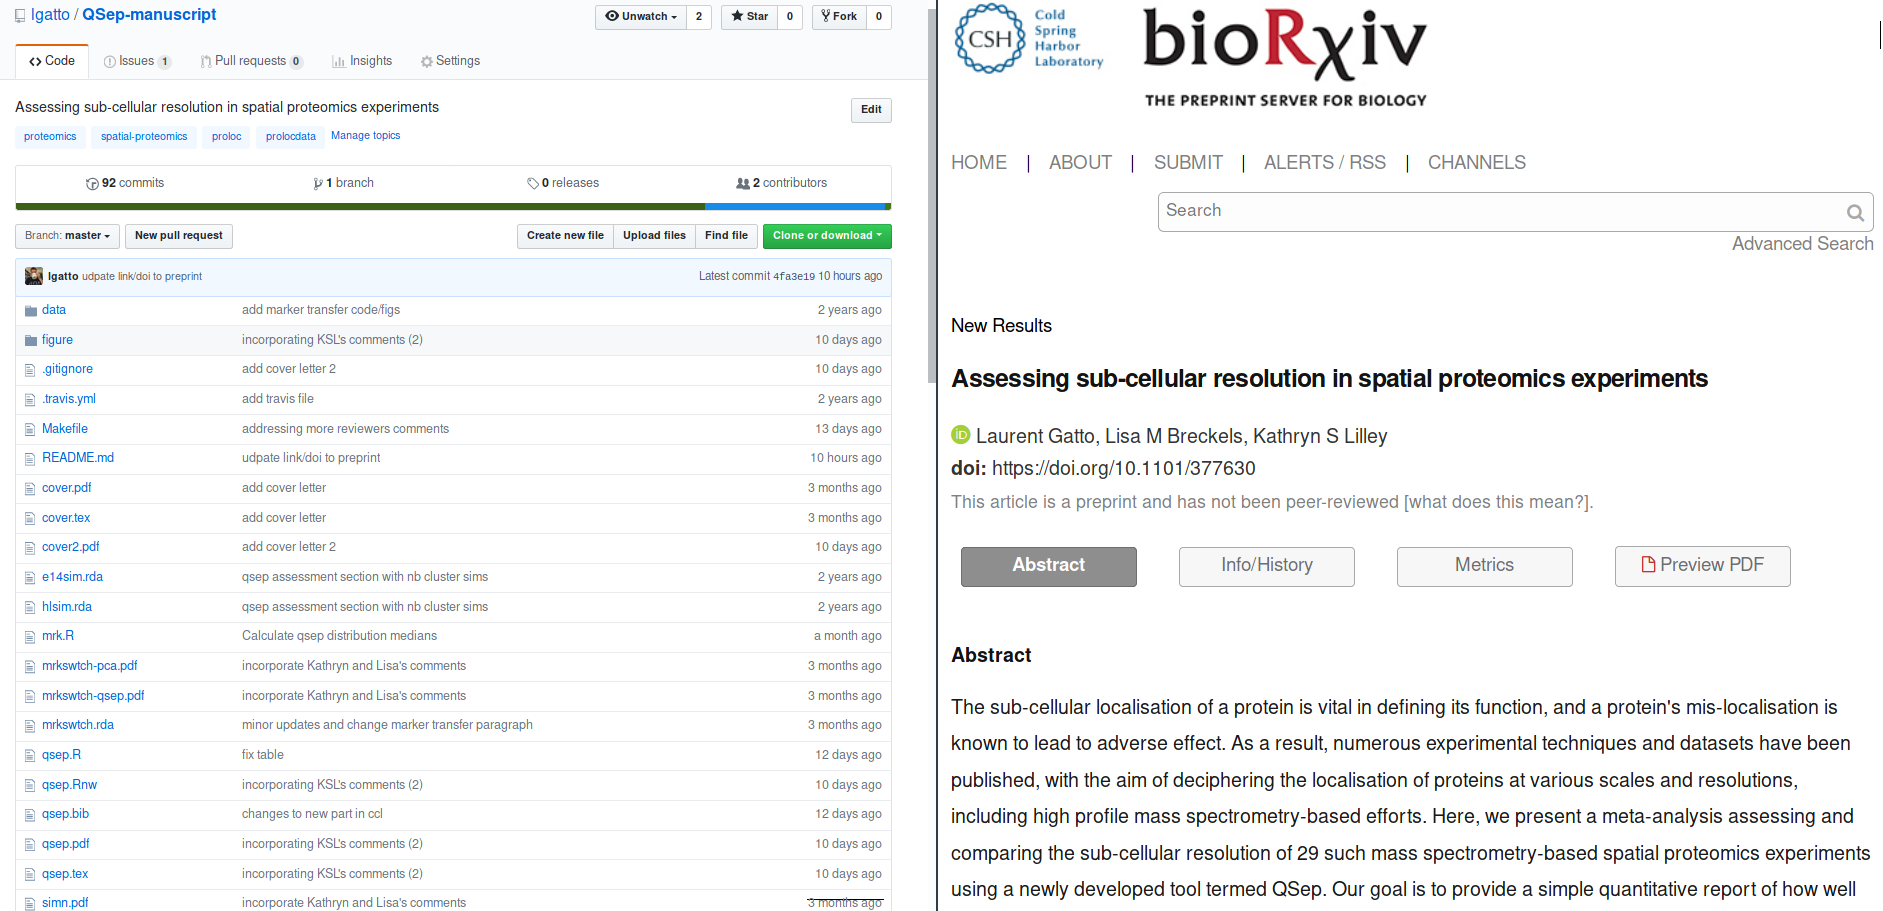
\includegraphics[width=1\linewidth]{./figs_local/qsep_screen.png}
    \caption{\url{https://github.com/lgatto/QSep-manuscript} and
      \url{https://doi.org/10.1101/377630} \citep{Gatto:2018}. In
      press in \textit{Current Opinions in Chemical Biology} now.}
  \end{figure}
\end{frame}

\begin{frame}{}
Working with open and reproducible research in mind doesn't mean
releasing everything prematurely, it means

\begin{itemize}
\item managing research in a way one can find data and results at
  every stage

\item one can reproduce results, re-run/compare them with new data or
  different methods/parameters, and

\item  one can release data (or parts thereof) when/if appropriate.
\end{itemize}
\end{frame}
